% Provenance (never printed): see sources/outline_sources.md (Year 2: natural hazards and risks
% quantified --- recurrence, probabilistic hazard, slope stability, tsunamis, floods, warning).
% Terminology from the UN report A/71/644 (UNDRR); the 475-year convention from the USGS
% Earthquake Hazards 201 page; the ground-motion prediction equation of Boore, Joyner and Fumal
% (USGS Open-File Report 93-509); run-ups from the NOAA NCEI tsunami database; the 1999 Vargas
% debris flows from USGS Open-File Report 01-0144. Ledger rows in sources/ledger/book4.md;
% curves and numbers from figdata/bachelor-2/hazards.py and the Book 4 second-writer scratch
% calculator calc/ch28.py. Hazards are described and quantified physically only: no advice.
\chapter{地质灾害与风险}\label{ch:b2:geological-hazards}

按平均每 475 年超越一次的地面运动设计的建筑，
在 50 年的使用寿命内遭遇该运动的概率为十分之一。两种说法说的是同一个数，
只是从两个角度来读。在两者之间来回换算，正是灾害科学的日常工作。本章
建立相应的工具：稀有事件的概率、场地的\omterm{def:b2:geological-hazards:psha}{危险性曲线}、斜坡的
稳定性、海啸的速度与爬高、洪水的频率，以及决定
各类灾害能提供多少预警的物理规律。
% ledger: usgs:eh201-475

\begin{recall}
\textbf{从中学各分册中}：自然\omterm{def:b2:geological-hazards:risk}{灾害风险}、自然灾害与滑坡；脆弱性、
风险、预防与\omterm{def:b2:geological-hazards:risk}{灾害风险}图；海啸；洪水的\omterm{def:b2:geological-hazards:return}{重现期}，以及
排序公式 $T = (n + 1)/m$，适用于 $n$ 个年最大值的记录。\textbf{从本科一年级分册中}：
古登堡–里克特定律 $\log_{10} N(\geq M) = a - bM$ 及其 b 值；地震矩与
矩震级；孔隙流体压力、有效应力 $\sigma' = \sigma - u$ 以及库仑破裂准则
$\tau = c' + \sigma' \tan\varphi'$。\textbf{从\cref{ch:b2:eruptive-styles}中}：\omterm{def:b2:eruptive-styles:pdc}{火山碎屑
密度流}、\omterm{def:b2:eruptive-styles:lahar}{火山泥流}与\omterm{def:b2:eruptive-styles:tephra}{火山灰碎屑}降落。\textbf{从数学分册中}：泊松分布与
指数分布、正态分布及其分布函数 $\Phi$。
\textbf{从物理系列本科二年级分册中}：表面重力波的色散关系
$\omega^2 = gk\tanh(kh)$。
\end{recall}

\section{危险性、暴露度与风险}\label{sec:b2:geological-hazards:risk}

\begin{definition}[地质灾害、暴露度、灾害风险]\label{def:b2:geological-hazards:risk}
\emph{地质灾害}\index{地质灾害}是一种源于地球内部作用的过程或现象——
例如地震、喷发，或滑坡、\omterm{def:b2:geological-hazards:slope}{泥石流}等块体运动——
它可能造成人员伤亡、受伤、财产损失或社会功能中断。它的特征是
发生地点、强度或震级，以及频率或概率。
\emph{暴露度}\index{暴露度（对某种灾害）}是指位于灾害可能波及范围内的人员、
建筑、基础设施及其他资产的状况，以其
数量或价值衡量。\emph{灾害风险}\index{灾害风险}是指潜在的生命损失，
健康或资产损失，可能发生于给定时段内，由
灾害、暴露度与受灾对象的脆弱性共同决定，并以概率方式确定。
\end{definition}
% ledger: undrr:hazard, undrr:geological, undrr:exposure, undrr:disaster-risk, undrr:vulnerability

国际术语体系将海啸单独归类：它由地震及其他
地质事件引发，成为一种海洋过程，并以沿岸、与水有关的灾害形式出现。
本章与其他灾害一并讨论，因为它们的源头是地质的。
% ledger: undrr:geological

该定义包含一个乘积关系。若强度为 $i$ 的事件以年发生率
$\lambda_i$ 出现，暴露资产价值为 $E$，且强度为 $i$ 的事件摧毁其中
比例为 $V_i$ 的部分（即脆弱性，介于 0 与 1 之间），则年均期望损失为
\begin{equation}
L = \sum_i \lambda_i \, E \, V_i ,
\label{eq:b2:geological-hazards:loss}
\end{equation}
通常简写为风险 = 危险性 $\times$ \omterm{def:b2:geological-hazards:risk}{暴露度} $\times$ 脆弱性。任一因子为零时，
风险即消失：一座猛烈喷发的火山位于无人岛屿上，一座人口稠密的城市位于安静的\omterm{def:b2:precambrian-earth:craton}{克拉通}上，或
建筑能够抵御震动。灾害科学测量的是第一个因子，下图
将它置于三者之中。

\begin{omfigure}
\centering
\begin{tikzpicture}[font=\small]
\fill[omThm!14] (90:1.05) circle (1.55);
\fill[omDef!14] (210:1.05) circle (1.55);
\fill[black!8] (330:1.05) circle (1.55);
\begin{scope}
\clip (90:1.05) circle (1.55);
\clip (210:1.05) circle (1.55);
\fill[omThm!45!omDef!45] (330:1.05) circle (1.55);
\end{scope}
\draw[omThm, thick] (90:1.05) circle (1.55);
\draw[omDef, thick] (210:1.05) circle (1.55);
\draw[black!60, thick] (330:1.05) circle (1.55);
\node[align=center, anchor=south] at (0,2.65) {\textbf{危险性} {\scriptsize（发生率 $\lambda_i$，强度）}};
\node[align=right, anchor=east] at (-2.55,-1.35) {\textbf{暴露度}\\[-1pt]{\scriptsize 资产 $E$}};
\node[align=left, anchor=west] at (2.55,-1.35) {\textbf{脆弱性}\\[-1pt]{\scriptsize 损失比例 $V_i$}};
\node[align=center, font=\scriptsize\bfseries] at (0,0) {风险};
\end{tikzpicture}
\par\smallskip{\small \omterm{def:b2:geological-hazards:risk}{灾害风险}的三个因子。期望损失仅在三者同时重叠之处非零：
即灾害波及暴露在外、且可能受到伤害的对象。}
\end{omfigure}

\section{稀有事件的概率}\label{sec:b2:geological-hazards:probability}

\begin{definition}[重现期]\label{def:b2:geological-hazards:return}
设某类事件——例如超过某一流量的洪水、超过某一水平的地面运动、
超过某一震级的地震——以平均年发生率 $\lambda$ 出现。其
\emph{重现期}\index{重现期}为 $T = 1/\lambda$：两次此类事件之间的平均间隔，
是其年发生率的倒数，而不是时刻表。
\end{definition}
% ledger: usgs:eh201-475

\begin{definition}[超越概率]\label{def:b2:geological-hazards:poisson}
某一水平在暴露时间 $t$ 内的\emph{超越概率}\index{超越概率}，
是指该水平在 $t$ 内至少被达到或超过一次的概率。
\end{definition}

\begin{proposition}[泊松复发模型]\label{prop:b2:geological-hazards:poisson}
假设事件一次只发生一个\index{泊松复发模型}，彼此独立，
且与已经过的时间无关，平均发生率为常数 $\lambda = 1/T$。则事件个数 $N$
在时间 $t$ 内服从均值为 $\lambda t$ 的泊松分布；时间
$t$ 内的\omterm{def:b2:geological-hazards:poisson}{超越概率}为
\begin{equation}
P(t) = 1 - e^{-t/T};
\label{eq:b2:geological-hazards:poisson}
\end{equation}
相邻两次事件的间隔服从均值为 $T$ 的指数分布。
\end{proposition}

\begin{proof}
设 $P_k(t)$ 为 $k$ 次事件落在 $[0, t]$ 内的概率。在很短的时间间隔 $\mathrm{d}t$ 内，
一次事件发生的概率为 $\lambda\,\mathrm{d}t$，与过去无关，发生两次的
概率为高阶无穷小。于是 $P_0(t + \mathrm{d}t) = P_0(t)(1 - \lambda\,\mathrm{d}t)$，即
$P_0' = -\lambda P_0$，$P_0(0) = 1$，故 $P_0(t) = e^{-\lambda t}$，且 $P(t) = 1 - P_0(t)$。同理
$P_k' = \lambda(P_{k-1} - P_k)$（$k \geq 1$），用归纳法求解：
$P_k(t) = (\lambda t)^k e^{-\lambda t}/k!$，即均值为 $\lambda t$ 的泊松分布。从某次事件
发生起算，同样的论证给出下一次事件晚于 $t$ 发生的概率：
$e^{-\lambda t}$，即指数分布的生存函数，其均值为
$\int_0^\infty e^{-\lambda t}\,\mathrm{d}t = 1/\lambda = T$。
\end{proof}

两个结论被普遍使用。若概率 $p$ 对应暴露时间 $t$，则\omterm{def:b2:geological-hazards:return}{重现期}
为 $T = -t/\ln(1 - p)$：50 年内 \qty{10}{\percent} 的概率，则 $T = 50/0.10536 =
474.6$ 年，即建筑规范中的“475 年”地震动，而 \qty{2}{\percent} 在 50 年内则
对应 2475 年。当 $t \ll T$ 时，$P \approx t/T$，发生率可读作每年的
概率。另一方面，在一个完整的\omterm{def:b2:geological-hazards:return}{重现期}内，概率为 $1 - e^{-1} =
\qty{63}{\percent}$，而非 1。下图（左）画出 \eqref{eq:b2:geological-hazards:poisson} 的
三个\omterm{def:b2:geological-hazards:return}{重现期}下的曲线。
% ledger: usgs:eh201-475
% values: T 474.561 and 2474.92 years; P(50|475) 0.0999 (hazards.py numbers)

该模型是否成立？全球震级不小于 7 的地震目录共有 696 次事件，
时间跨度为 1976 年至 2025 年，共 695 个间隔，平均间隔为 26.2 天。若它们构成泊松过程，
则间隔长于 $t$ 的比例应为 $e^{-t/26.2}$，在对数
坐标轴上为一条直线。下图（右）表明情况近似如此：间隔超过 30 天的占 \qty{30.4}{\percent}，
模型的相应值为 \qty{31.8}{\percent}，间隔的标准差
为均值的 1.07 倍，模型中则恰为 1。偏差出现在短间隔处：有 36 对
事件发生在同一天，即余震与双震，无记忆过程不会使其聚集。危险性
图因此从目录中剔除相依事件（去聚集化），使
剩下的主震可视为泊松过程；它们按震级的速率来自
古登堡–里克特定律。
% ledger: data:usgs-comcat, usgs:eh201-poisson
% values: m7_events 696, mean 26.2245 d, cv 1.06891, same-day 36, frac>30 d 0.303597 vs 0.318552

\begin{omfigure}
\centering
\begin{minipage}[b]{0.49\linewidth}\centering
\begin{tikzpicture}
\begin{axis}[omrecord, width=0.96\linewidth, height=5.2cm, xmin=0, xmax=200, ymin=0, ymax=1,
  xlabel={暴露时间 $t$（年）}, ylabel={超越概率},
  tick label style={font=\scriptsize}, label style={font=\small},
  xtick={0,50,100,150,200}, ytick={0,0.2,...,1}]
% computed in figdata/bachelor-2/hazards.py part poisson
\addplot[omThm, line width=1pt] table[x=t_yr, y=P50] {figdata/out/bachelor-2-hazards-poisson.dat};
\addplot[omDef, line width=1pt] table[x=t_yr, y=P475] {figdata/out/bachelor-2-hazards-poisson.dat};
\addplot[black!70, line width=1pt, densely dashed] table[x=t_yr, y=P2475] {figdata/out/bachelor-2-hazards-poisson.dat};
\draw[black!50, densely dotted] (axis cs:50,0) -- (axis cs:50,1);
\fill[omDef] (axis cs:50,0.1) circle (1.8pt);
\node[font=\scriptsize, text=omThm, anchor=west] at (axis cs:62,0.86) {$T = 50$};
\node[font=\scriptsize, text=omDef, anchor=west] at (axis cs:120,0.34) {$T = 475$};
\node[font=\scriptsize, text=black!70, anchor=west] at (axis cs:120,0.12) {$T = 2475$};
\node[font=\scriptsize, anchor=west, text=omDef] at (axis cs:52,0.2) {\qty{10}{\percent}};
\end{axis}
\end{tikzpicture}
\end{minipage}\hfill
\begin{minipage}[b]{0.49\linewidth}\centering
\begin{tikzpicture}
\begin{axis}[omrecord, width=0.93\linewidth, height=5.2cm, xmin=0, xmax=120, ymode=log,
  ymin=0.008, ymax=1.1, xlabel={间隔 $t$（天）}, ylabel={间隔 $> t$ 的比例},
  tick label style={font=\scriptsize}, label style={font=\small}, xtick={0,30,60,90,120},
  legend style={at={(0.03,0.03)}, anchor=south west, font=\scriptsize, draw=black!30},
  legend cell align=left]
% computed in figdata/bachelor-2/hazards.py part survival; ledger: data:usgs-comcat
\addplot[omThm, only marks, mark=*, mark size=1.2pt] table[x=t_day, y=observed] {figdata/out/bachelor-2-hazards-survival.dat};
\addlegendentry{$M \geq 7$，1976--2025 年}
\addplot[black, line width=0.9pt] table[x=t_day, y=poisson] {figdata/out/bachelor-2-hazards-survival.dat};
\addlegendentry{泊松过程，平均间隔 26.2 天}
\end{axis}
\end{tikzpicture}
\end{minipage}
\par\smallskip{\small 左图：暴露时间 $t$ 内至少发生一次事件的概率，对
\omterm{def:b2:geological-hazards:return}{重现期}为 50、475 和 2475 年的情形；475 年\omterm{def:b2:geological-hazards:return}{重现期}事件在 50 年内的概率为
\qty{10}{\percent}。右图：1976--2025 年全球目录中，震级不小于 7 的 696 次地震之间的
间隔，与同速率泊松过程的指数律相比较。数据：
USGS ANSS 综合目录。}
\end{omfigure}

\section{地震危险性}\label{sec:b2:geological-hazards:seismic}

\begin{definition}[概率地震危险性分析，地震动预测方程，峰值地面加速度，危险性曲线]\label{def:b2:geological-hazards:psha}
某地点的\emph{峰值地面加速度}\index{峰值地面加速度}（PGA）是地震期间地面最大的
水平加速度的绝对值，通常以
$g$ 的分数表示。\emph{地震动预测方程}\index{地震动预测方程}（GMPE）给出
某地点震动量（如 PGA）的概率分布，即
中位数与离散度，它是震级、到震源距离和场地条件的函数。
\emph{概率地震危险性分析}\index{概率地震危险性分析}（PSHA）将所有可能影响
某地点的地震，连同其发生率与距离，结合 GMPE，给出各震动水平被超越的
年速率。该速率对震动水平作图所得的曲线，
即为该地点的\emph{危险性
曲线}\index{危险性曲线}。
\end{definition}
% ledger: usgs:eh201-pga, usgs:eh201-475

PGA 即地面某一质点所经历的加速度。建筑物响应的是地震动中
与其自身固有周期相近的部分，规范也绘制这种响应，即谱加速度；
PGA 使推理简单，故此处采用。
% ledger: usgs:eh201-pga

\begin{method}[概率地震危险性分析]\label{met:b2:geological-hazards:psha}
\begin{enumerate}
  \item \textbf{震源区。}标出场地周围的断层和震源区，并给出
        它们各自到场地的距离 $d$。
  \item \textbf{复发。}对每个震源区，取各震级地震的年发生率，
        由古登堡–里克特定律给出，并在最大震级 $M_{\max}$ 处截断：
        $N(\geq m) = 10^{a - bm} - 10^{a - bM_{\max}}$，从最小震级 $M_{\min}$ 起算。
        将震级范围切分为若干段，每段速率为 $\nu_j$，震级在 $m_j$ 附近。
  \item \textbf{地震动。}由 GMPE 取各段的中位数 $\mu_j = \log_{10}\mathrm{PGA}$ 和
        各段的离散度 $\sigma$；PGA 超过 $a$ 的概率为
        $1 - \Phi\bigl((\log_{10} a - \mu_j)/\sigma\bigr)$。
  \item \textbf{求和。}超过 $a$ 的年超越率为 $\lambda(a) = \sum_j \nu_j
        \bigl[1 - \Phi\bigl((\log_{10} a - \mu_j)/\sigma\bigr)\bigr]$，对所有震源区求和。
  \item \textbf{读取。}\omterm{def:b2:geological-hazards:poisson}{超越概率}为 $p$、时间为 $t$ 年的 PGA，即满足
        $\lambda(a) = -\ln(1 - p)/t$：\num{2.107e-3} 每年，对应 50 年内 \qty{10}{\percent} 的概率。
\end{enumerate}
\end{method}

本章所用的 GMPE 为博尔、乔伊纳与富马尔所给出，由 271 条记录拟合，这些记录取自 20
次地震（北美西部）。对随机水平分量，以 $g$ 为单位，
\begin{equation}
\log_{10}\mathrm{PGA} = -0.105 + 0.229\,(M - 6) - 0.778\log_{10} r + 0.162\,G_B + 0.251\,G_C,
\qquad r = \sqrt{d^2 + 5.57^2},
\label{eq:b2:geological-hazards:gmpe}
\end{equation}
其中 $M$ 为矩震级，$d$ 为到断层破裂面地表投影的距离（千米），
$\sigma = 0.230$ 为中位数附近的离散度。该式适用于 $5.0 \leq M \leq 7.7$ 且 $d
\leq \qty{100}{km}$。常数 \qty{5.57}{km} 为回归拟合得到的虚拟深度，
它使震源上方的地震动保持有限。震级 6、距离 \qty{15}{km} 处的中位数为
\qty{0.091}{g}，震级 7.5 时为 \qty{0.200}{g}；一个标准差使
中位数乘以或除以 $10^{0.230} = 1.70$。
% ledger: bjf93:pga, bjf97:pga-ln
% values: M6@15 km 0.0908 g, M7.5@15 km 0.2003 g (hazards.py numbers)

$G_B$ 与 $G_C$ 两项反映场地效应。场地按上部 \qty{30}{m} 的平均剪切
波速分类：A 类为高于 \qty{750}{m.s^{-1}}（$G_B = G_C = 0$），B 类为
360 至 \qty{750}{m.s^{-1}}（$G_B = 1$），C 类为 180 至 \qty{360}{m.s^{-1}}（$G_C = 1$）。软
土场地使岩石地震动放大：B 类为 $10^{0.162} = 1.45$ 倍，C 类
为 $10^{0.251} = 1.78$ 倍。波进入较慢的介质时，速度减小、波长变短、振幅增大，软弱层或
充填沉积物的盆地可能产生共振并将其困住。
% ledger: bjf93:pga

下图将该方法应用于距岩石场地 \qty{15}{km} 的单一震源区，取 $a
= 4.0$、$b = 1.0$、$M_{\min} = 5$ 与 $M_{\max} = 7.5$：每年约 0.1 次
震级 5 级及以上的地震。PGA 很小时，曲线趋于该速率，因为每次地震都会超过一个较弱的
水平。50 年内 \qty{10}{\percent} 对应的 PGA 为 \qty{0.22}{g}。若每次地震恰好产生其中位数，
则同样的速率将在 \qty{0.13}{g} 处即已达到，而高于
最大地震中位数（\qty{0.20}{g}）的任何水平都不可能被超过。离散度主导了罕见
水平：\omterm{def:b2:geological-hazards:return}{重现期} 475 年的地震动主要来自中等地震，这些地震的震动强于其
中位数。
% values: psha_rate_m5 0.0997, psha_pga475 0.220894, psha_pga475_median 0.125607, median M7.5 0.2003 (hazards.py numbers)

\begin{omfigure}
\centering
\begin{tikzpicture}
\begin{axis}[omrecord, width=0.8\linewidth, height=5.6cm, xmode=log, ymode=log, xmin=0.01,
  xmax=2, ymin=1e-6, ymax=0.3, xlabel={峰值地面加速度（\unit{g}）},
  ylabel={年超越率}, unbounded coords=jump,
  tick label style={font=\scriptsize}, label style={font=\small},
  xtick={0.01,0.03,0.1,0.3,1}, xticklabels={0.01,0.03,0.1,0.3,1},
  legend style={at={(0.03,0.03)}, anchor=south west, font=\scriptsize, draw=black!30},
  legend cell align=left]
% computed in figdata/bachelor-2/hazards.py part psha; ledger: bjf93:pga
\addplot[omThm, line width=1.2pt] table[x=pga_g, y=rate] {figdata/out/bachelor-2-hazards-psha.dat};
\addlegendentry{计入 GMPE 离散度}
\addplot[black!60, line width=1pt, densely dashed] table[x=pga_g, y=rate_median] {figdata/out/bachelor-2-hazards-psha.dat};
\addlegendentry{仅中位数}
\draw[omDef, densely dotted, thick] (axis cs:0.01,2.107e-3) -- (axis cs:2,2.107e-3);
\draw[omDef, densely dotted, thick] (axis cs:0.2209,1e-6) -- (axis cs:0.2209,2.107e-3);
\node[font=\scriptsize, text=omDef, anchor=south east] at (axis cs:2,2.107e-3) {50 年内 \qty{10}{\percent}};
\node[font=\scriptsize, text=omDef, anchor=west] at (axis cs:0.235,2e-5) {\qty{0.22}{g}};
\end{axis}
\end{tikzpicture}
\par\smallskip{\small \omterm{def:b2:geological-hazards:psha}{危险性曲线}：岩石场地 PGA 超过各
水平的年速率，针对距离 \qty{15}{km} 的单一震源区（截断的古登堡–里克特复发关系，$b = 1$，
震级 5 至 7.5），并采用博尔、乔伊纳和富马尔的 GMPE。点线用于读出
\qty{10}{\percent}（50 年内）对应的水平。不计离散度时（虚线），曲线止于
最大地震的中位地震动。}
\end{omfigure}

\section{火山灾害}\label{sec:b2:geological-hazards:volcanic}

火山通过几种同时发生的过程造成威胁，各过程有各自的影响范围：\omterm{def:b2:eruptive-styles:tephra}{火山灰碎屑}
顺风远落，\omterm{def:b2:eruptive-styles:pdc}{火山碎屑密度流}与\omterm{def:b2:eruptive-styles:lahar}{火山泥流}沿山谷流动，熔岩流推进较慢
（见\cref{ch:b2:eruptive-styles}）。\omterm{def:b2:geological-hazards:risk}{灾害风险}图为每种过程划定一区，依据过去喷发的
堆积物及流动与降落模型。火山概率的构造方式不同于
地震，因为苏醒中的火山并非平稳过程。事件树由
活动异常出发，经分支通向各种结果，每一分支都由必要的前一事件通向更具体的
结果——活动异常是否为\omterm{def:b2:magma-emplacement:magma}{岩浆}性；是否喷发；喷发为爆炸式或溢流式；\omterm{def:b2:eruptive-styles:pdc}{火山碎屑流}
是否到达某一山谷。结果的概率等于沿其分支的
条件概率之积。设 $M$ 为\omterm{def:b2:magma-emplacement:magma}{岩浆}性活动异常，$E$ 为喷发，$X$ 为\omterm{def:b2:eruptive-styles:regimes}{爆炸式
喷发}，$V$ 为流入山谷的\omterm{def:b2:eruptive-styles:pdc}{火山碎屑流}，
\begin{equation*}
P(V) = P(M) \, P(E \mid M) \, P(X \mid E) \, P(V \mid X),
\end{equation*}
各因子依据该火山的过去活动、类似火山或模型估计，并用
贝叶斯定理随新监测数据到来而修正（见\cref{exo:b2:geological-hazards:8}）。
% ledger: nh02:event-tree

\section{滑坡}\label{sec:b2:geological-hazards:landslides}

斜坡只要其物质沿任一可能滑动面上的强度
超过重力在该面上施加的应力。强度即本科一年级
分册中的库仑破裂准则，以有效应力写出：孔隙中的水承担部分法向荷载，
并降低摩擦力。

\begin{definition}[安全系数、泥石流]\label{def:b2:geological-hazards:slope}
斜坡沿某一潜在滑动面的\emph{安全系数}\index{安全系数} $F$，
为该面上可用抗剪强度与维持
平衡所需切应力之比。斜坡在 $F > 1$ 时稳定，$F$ 降至 1 时破坏。一种
\emph{泥石流}\index{泥石流}是饱水的泥、沙、砾石、块石和木材的快速流动，
沿河道作为一个致密整体向下运动，颗粒承担其大部分重量，并
在河道出口的扇形堆积体上铺展。
\end{definition}

\begin{proposition}[无限边坡]\label{prop:b2:geological-hazards:infinite-slope}
单位重为 $\gamma$、竖向厚度为 $z$ 的一层土，覆于滑动面之上，
该滑动面与地面平行，倾角为 $\beta$；其强度参数为 $c'$ 与 $\varphi'$，且
滑动面上的孔隙压力为 $u = r_u \gamma z$。若土层足够长，使其两端可以
忽略，则
\begin{equation}
F = \frac{c' + \gamma z\,(\cos^2\beta - r_u)\tan\varphi'}{\gamma z \sin\beta\cos\beta}.
\label{eq:b2:geological-hazards:infinite-slope}
\end{equation}
对于干燥、无内聚力的土层，$F = \tan\varphi'/\tan\beta$：它可稳定至 $\beta = \varphi'$。
\end{proposition}

\begin{proof}
取水平宽度为 $b$ 的土柱，其重量为 $W = \gamma z b$（每单位长度，垂直于剖面），
其底面与坡面平行，长度为 $b/\cos\beta$。柱体两侧所受的力
在无限边坡中大小相等、方向相反而抵消。将 $W$ 沿底面法向与
切向分解，并除以底面长度，则底面上的法向应力与切应力分别为
$\sigma = \gamma z\cos^2\beta$ 与 $\tau = \gamma z \sin\beta\cos\beta$。有效法向应力
为 $\sigma' = \sigma - u = \gamma z(\cos^2\beta - r_u)$，可用强度为 $c' +
\sigma'\tan\varphi'$，$F$ 即二者之比。当 $c' = 0$ 且 $r_u = 0$ 时，$F = \cos^2\beta
\tan\varphi'/(\sin\beta\cos\beta) = \tan\varphi'/\tan\beta$.
\end{proof}

\begin{omfigure}
\centering
\begin{minipage}[b]{0.49\linewidth}\centering
\begin{tikzpicture}[scale=0.82, font=\scriptsize]
\def\t{0.57735}
\fill[black!10] (0,-1) -- (5.6,{5.6*\t-1}) -- (5.6,-1.6) -- (0,-1.6) -- cycle;
\fill[omThm!12] (0,0) -- (5.6,{5.6*\t}) -- (5.6,{5.6*\t-1}) -- (0,-1) -- cycle;
\draw[thick] (0,0) -- (5.6,{5.6*\t});
\draw[omDef, densely dashed] (0,-0.4) -- (5.6,{5.6*\t-0.4});
\draw[omThm, very thick] (0,-1) -- (5.6,{5.6*\t-1});
\fill[white, opacity=0.55] (2.4,{2.4*\t}) -- (3.2,{3.2*\t}) -- (3.2,{3.2*\t-1}) -- (2.4,{2.4*\t-1}) -- cycle;
\draw[black!75] (2.4,{2.4*\t}) -- (3.2,{3.2*\t}) -- (3.2,{3.2*\t-1}) -- (2.4,{2.4*\t-1}) -- cycle;
\draw[->, thick] (2.8,{2.8*\t-0.3}) -- (2.8,{2.8*\t-1.35}) node[below] {$W$};
\draw[<->] (4.6,{4.6*\t-1}) -- (4.6,{4.6*\t}) node[midway, right] {$z$};
\draw[black!60] (0.25,-1) -- (1.45,-1);
\draw[black!60] (1.25,-1) arc (0:30:1.0);
\node at (1.55,-0.78) {$\beta$};
\node[omDef, anchor=north, rotate=30, inner sep=1.5pt] at (1.3,{1.3*\t-0.4}) {地下水位};
\node[omThm, anchor=north, rotate=30] at (4.4,{4.4*\t-1.05}) {滑动面};
\end{tikzpicture}
\end{minipage}\hfill
\begin{minipage}[b]{0.49\linewidth}\centering
\begin{tikzpicture}
\begin{axis}[omrecord, width=0.97\linewidth, height=5.2cm, xmin=0, xmax=0.5, ymin=0.5, ymax=2,
  xlabel={孔隙压力比 $r_u$}, ylabel={安全系数 $F$},
  tick label style={font=\scriptsize}, label style={font=\small}, xtick={0,0.1,...,0.5},
  /pgf/number format/fixed]
% computed in figdata/bachelor-2/hazards.py part slope
\addplot[omDef, line width=1pt] table[x=r_u, y=F25] {figdata/out/bachelor-2-hazards-slope.dat};
\addplot[black, line width=1pt] table[x=r_u, y=F30] {figdata/out/bachelor-2-hazards-slope.dat};
\addplot[omThm, line width=1pt] table[x=r_u, y=F35] {figdata/out/bachelor-2-hazards-slope.dat};
\draw[black!50, densely dashed] (axis cs:0,1) -- (axis cs:0.5,1);
\node[font=\scriptsize, text=omDef, anchor=south west] at (axis cs:0.02,1.80) {\ang{25}};
\node[font=\scriptsize, anchor=south west] at (axis cs:0.02,1.50) {\ang{30}};
\node[font=\scriptsize, text=omThm, anchor=north west] at (axis cs:0.01,1.19) {\ang{35}};
\node[font=\scriptsize, text=black!60, anchor=north east] at (axis cs:0.5,0.98) {失稳};
\end{axis}
\end{tikzpicture}
\end{minipage}
\par\smallskip{\small 左：无限边坡，厚度为 $z$ 的土层位于
与地面平行的滑动面上，土柱重为 $W$。右：各坡角下的\omterm{def:b2:geological-hazards:slope}{安全系数}随
孔隙压力比的变化，取 $c' = \qty{5}{kPa}$，$\varphi' = \ang{35}$，$\gamma = \qty{19}{kN.m^{-3}}$，$z =
\qty{2}{m}$。三条曲线分别对应三个坡角。孔隙压力升高使各斜坡失稳。}
\end{omfigure}
% values: F(r_u = 0) 1.845, 1.517, 1.280; r_u at F = 1: 0.462, 0.320, 0.188 (calc/ch28.py)

式\eqref{eq:b2:geological-hazards:infinite-slope}指出了两种常见的触发因素：降雨
抬高地下水位并使 $r_u$ 增大；$F$ 随 $r_u$ 线性下降，因此干燥时安全的斜坡，
湿润时便会失稳：在上图中，\ang{35} 的斜坡在 $r_u = 0.19$ 时失稳，
\ang{25} 的斜坡则只在 0.46 时失稳。地震动附加一水平力，记为 $kW$，$k$ 为
$g$ 的一个分数，则分子减少 $\gamma z k \sin\beta\cos\beta\tan\varphi'$，分母增加
$\gamma z k\cos^2\beta$——一种拟静力分析，在本阶段不加证明地承认，它
以一个稳定的力代替短暂的地震动。内聚力项 $c'/(\gamma z\sin\beta\cos\beta)$
随土层加厚而减小，因此内聚力对薄层土的保护作用强于深层土。

1999 年 12 月，一场持续三天的风暴在卡拉卡斯以北海岸的迈凯蒂亚降下 \qty{911}{mm} 降雨量。
数以千计的浅层滑坡发生在阿维拉山脉的斜坡上，
坡角从 \ang{30} 到超过 \ang{60} 不等，平均为 \ang{42}。在河道中，它们汇合
成为\omterm{def:b2:geological-hazards:slope}{泥石流}，流速为 3 至 \qty{14}{m.s^{-1}}，弯道处表面超高，
并搬运长达 \qty{11}{m} 的巨石。在下图所示的卡拉瓦列达冲积扇上，它们
留下厚达 \qty{6}{m} 的巨石碎屑，约 180 万立方米。死亡人数
通常给出的数字约为 \num{30000}。
% ledger: vargas:storm, vargas:slopes, vargas:velocity, vargas:caraballeda, vargas:deaths

\begin{omfigure}
\centering
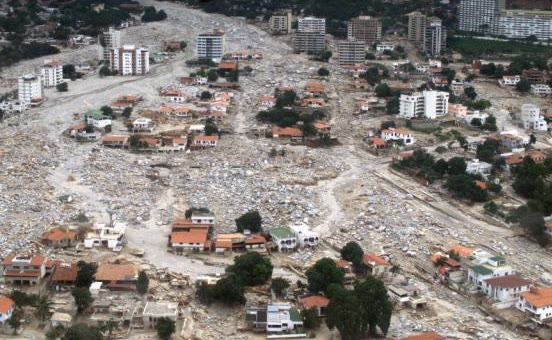
\includegraphics[width=0.62\linewidth]{images/book4/b2-28-caraballeda-debris-flow.jpg}
\par\smallskip{\small 委内瑞拉海岸，卡拉瓦列达冲积扇上的\omterm{def:b2:geological-hazards:slope}{泥石流}堆积，
形成于 1999 年 12 月风暴之后：\omterm{def:b2:geological-hazards:slope}{泥石流}离开主河道，将小镇埋入
巨石之下。照片：Lawson Smith, U.S. Army Corps of Engineers（公有领域）。}
\end{omfigure}
% ledger: photo:b2-28-caraballeda, vargas:caraballeda

\section{海啸}\label{sec:b2:geological-hazards:tsunamis}

由海底突然隆升引发的海啸，波长为数十至数百
千米，远大于海洋深度。它是长波，其速度只取决于
水深。

\begin{proposition}[长波]\label{prop:b2:geological-hazards:long-waves}
波长远大于水深 $h$ 的表面重力波，以
$c = \sqrt{gh}$ 的速度传播，与波长无关。若它缓慢进入较浅的水域，
且不发生反射或破碎，其振幅 $A$ 按 $h^{-1/4}$ 增长。
\end{proposition}

\begin{proof}
由色散关系可得相速度 $c = \omega/k = \sqrt{(g/k)\tanh(kh)}$。对长波，
有 $kh = 2\pi h/\lambda \ll 1$，且 $\tanh(kh) \approx kh$，于是 $c = \sqrt{gh}$，与
$k$ 无关，即长波不发生频散。单位海面面积上的波能为 $\frac12
\rho g A^2$，并以 $c$ 传播。若能量无反射或损失，则通量 $\frac12\rho g A^2
c$ 经过任一截面时沿路径保持不变，即 $A^2 \sqrt{h}$ 为常数，且 $A \propto
h^{-1/4}$。
\end{proof}

水深超过 \qty{4000}{m} 时，海啸以 \qty{198}{m.s^{-1}}（即 \qty{713}{km/h}）传播；
在超过 \qty{5000}{m} 的水深处为 \qty{797}{km/h}，即预警机构引用的“超过 800 km/h”。
靠近海岸、水深 \qty{10}{m} 处，它减速至 \qty{36}{km/h}；其波前
被后方的水追上，波长变短、变陡，波高增大。
% ledger: nws:tsunami-speed

\begin{definition}[海啸爬高]\label{def:b2:geological-hazards:tsunami}
海岸某一点的\emph{海啸爬高}\index{海啸爬高}，是指该处
水向内陆所能到达的最高地面相对于当时海平面的高度。
从岸线到该点的水平距离即为淹没距离。
\end{definition}

每次海啸之后，调查队依据水痕、碎屑线和破坏痕迹测量爬高。
全球海啸数据库收录了 \num{2177} 条爬高观测，针对
2004 年 12 月 26 日的印度洋海啸，由苏门答腊近海震级 9.1 的地震引发，最大水高为
\qty{50.9}{m}；另有 \num{6429} 条观测对应 2011 年 3 月 11 日本州近海的海啸，震级同为 9.1，
其最大值为 \qty{39.3}{m}。两次海啸分别造成 \num{227899} 人和 \num{18423} 人死亡。在班达亚齐
海水漫至下方清真寺二楼的中部。
% ledger: ncei:tsu-2004, ncei:tsu-2011, usgs:aceh-mosque

\begin{omfigure}
\centering
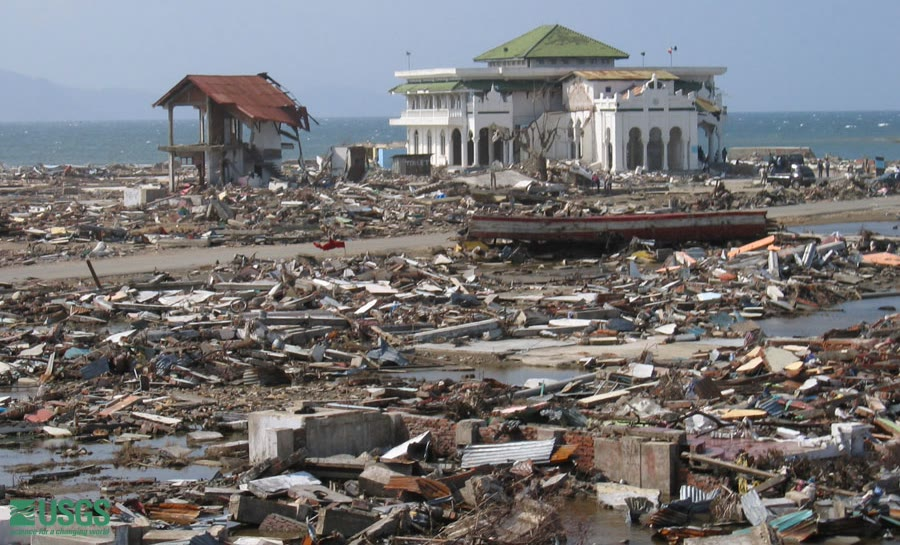
\includegraphics[width=0.62\linewidth]{images/book4/b2-28-aceh-mosque-tsunami.jpg}
\par\smallskip{\small 苏门答腊班达亚齐，2005 年 1 月 21 日，2004 年 12 月 26 日海啸之后：
一座清真寺矗立在周围建筑的瓦砾之中。图片来源：美国地质调查局
（公有领域）。}
\end{omfigure}
% ledger: photo:b2-28-aceh

\section{洪水}\label{sec:b2:geological-hazards:floods}

\begin{definition}[洪水频率曲线]\label{def:b2:geological-hazards:flood}
河流在某一水文站处的\emph{洪水频率曲线}\index{洪水频率曲线}，是年最大洪峰流量
关于其\omterm{def:b2:geological-hazards:return}{重现期}（或年\omterm{def:b2:geological-hazards:poisson}{超越概率}）的曲线，
由该站的年最大洪峰记录构成，通常还借助一个拟合的
概率律加以延伸。
\end{definition}

教科书中的秩公式确定了曲线上各点的位置，这一做法是有依据的。

\begin{proposition}[威布尔绘点位置]\label{prop:b2:geological-hazards:weibull}
设 $n$ 个年最大洪峰相互独立，且服从同一连续分布，并设
$G(x)$ 为某年洪峰超过 $x$ 的概率。按从大到小计数，第 $m$ 个洪峰
的期望\omterm{def:b2:geological-hazards:poisson}{超越概率}为 $m/(n + 1)$，因此它应绘于 $T = (n +
1)/m$ 处。
\end{proposition}

\begin{proof}
对连续分布，$U = G(X)$ 在 $[0, 1]$ 上服从均匀分布，且 $G$ 单调递减，故第
$m$ 大的洪峰对应于第 $m$ 小的值，这 $n$ 个均匀变量相互独立，
记为 $U_{(m)}$。其密度为 $f(u) = \frac{n!}{(m-1)!\,(n-m)!}u^{m-1}(1-u)^{n-m}$：$n$ 个值中有一个位于
$u$ 处，下方有 $m - 1$ 个，上方有 $n - m$ 个。利用贝塔积分 $\int_0^1 u^{p}(1-u)^{q}\,\mathrm{d}u
= p!\,q!/(p + q + 1)!$，
\begin{equation*}
\mathbb{E}[U_{(m)}] = \frac{n!}{(m-1)!\,(n-m)!}\cdot\frac{m!\,(n-m)!}{(n+1)!} = \frac{m}{n+1}. \qedhere
\end{equation*}
\end{proof}

因此，一条 30 年记录中最大的洪峰应绘于 31 年处，而记录本身无法确定
100 年一遇洪水。为此，需用极值律拟合洪峰，常用耿贝尔分布，
$\Pr(\text{洪峰} \leq x) = \exp\bigl(-e^{-(x - u)/\alpha}\bigr)$，其 $T$ 年一遇洪水为 $x_T = u
- \alpha\ln\bigl(-\ln(1 - 1/T)\bigr)$：对 $-\ln(-\ln(1 - 1/T))$ 作图呈一条直线，
外推至记录范围之外，风险随距离增大而增加。

\section{监测与预警}\label{sec:b2:geological-hazards:warning}

\begin{definition}[预警系统]\label{def:b2:geological-hazards:warning}
\emph{预警系统}\index{预警系统}是一个综合系统，集灾害监测、预报、风险评估、
信息传播与防范准备于一体，能够及时采取行动，
在危险事件发生之前。它包含四个要素：对风险的认识；灾害的检测、
监测与预报；预警信息的发布；以及
应对的准备。
\end{definition}
% ledger: undrr:ews

物理规律决定了每次预警能争取到多少时间。地震波无法被超越，但具有破坏性的
S 波在上地壳中约以 \qty{3.2}{km.s^{-1}} 的速度传播，而
P 波约为 \qty{5.8}{km.s^{-1}}：由震中附近最初几个 P 波算出的警报，会先于
S 波到达城市，提前量为 $d(1/3.2 - 1/5.8) = \qty{0.14}{s}$（每千米距离 $d$），再减去
检测与计算所需的时间。距离 \qty{100}{km} 的城市至多获得 \qty{14}{s}；在震源附近
存在盲区，无法获得预警（见\cref{exo:b2:geological-hazards:12}）。穿越 \qty{100}{km} 海域的海啸
若海深 \qty{2000}{m}，需 12 分钟；横跨大洋则需数小时。2011 年，日本的
预警在地震后约三分钟发出，但所估震级偏低，
原因是仪器饱和；约 28 分钟后，利用近海 GPS 浮标的数据对其进行了更新。
深海压力计每 15 秒将海底压力换算为
海面高度，现已能通过卫星报告经过的海啸。
% ledger: data:prem, jma:warning, ndbc:dart
% values: 0.1401 s/km, 14.0 s at 100 km; 140 m/s over 2000 m, 11.9 min per 100 km (calc/ch28.py)

\begin{inthefield}[观测斜坡的蠕动]
在已知会蠕动的斜坡上，监测团队安装仪器，测量无限斜坡方程中的
各个变量。钻孔中的孔隙水压计记录滑动面上的孔隙压力；
分段读取的测斜管显示地面在何处弯曲以及弯曲速率；GNSS
台站与伸长计记录地表位移；雨量计记录触发因素。
团队逐季比较位移与降雨量及水压，并
寻找先于破坏出现的加速现象。
\end{inthefield}

\section*{练习}\label{sec:b2:geological-hazards:exercises}

除另有说明外，练习数据如下：$g = \qty{9.81}{m.s^{-2}}$；水的重度
\qty{9.81}{kN.m^{-3}}；对岩石场地应用\omterm{def:b2:geological-hazards:psha}{地震动预测方程} \eqref{eq:b2:geological-hazards:gmpe}（$G_B = G_C = 0$），
$\sigma = 0.230$；上地壳中 P 波与 S 波速度分别为 5.8 和 \qty{3.2}{km.s^{-1}}。
结果保留三位有效数字。
% ledger: bjf93:pga, data:prem

\begin{exercise}[$\star$]\label{exo:b2:geological-hazards:1}
在泊松模型下：(a) 30 年内至少出现一次 100 年一遇洪水的概率是多少？
(b) 一个世纪内不出现 100 年一遇洪水的概率是多少？(c) 求
50 年内\omterm{def:b2:geological-hazards:poisson}{超越概率}为 \qty{5}{\percent} 的地震动的\omterm{def:b2:geological-hazards:return}{重现期}。
\end{exercise}

\begin{exercise}[$\star$]\label{exo:b2:geological-hazards:2}
两座城镇面临强烈震动。甲镇每 200 年发生一次此类震动，将
摧毁其 5000 栋建筑中的 \qty{2}{\percent}；乙镇每 50 年一次，摧毁
其 800 栋建筑中的 \qty{10}{\percent}。(a) 求每座城镇每年
平均被摧毁的建筑数。(b) 哪座城镇风险更大，尽管其\omterm{def:b2:geological-hazards:risk}{暴露度}较小？(c)
三个因素中哪一个造成了这种差异？
\end{exercise}

\begin{exercise}[$\star$]\label{exo:b2:geological-hazards:3}
(a) 求海啸在深度分别为 4000、200 和 \qty{10}{m} 时的传播速度。(b) 需多长时间才能穿越
\qty{1500}{km} 长、深 \qty{4000}{m} 的海域？(c) 在何种深度下，
海啸的传播速度为 \qty{800}{km/h}？
\end{exercise}

\begin{exercise}[$\star$]\label{exo:b2:geological-hazards:4}
一种干燥、无黏聚力的砂，内摩擦角 $\varphi' = \ang{33}$，形成一个长斜坡。(a) 求其
在 \ang{25} 处的\omterm{def:b2:geological-hazards:slope}{安全系数}。(b) 它能形成的最陡斜坡是多少？(c) 斜坡饱和，
地下水位位于地表，且渗流平行于坡面，故 $r_u = \gamma_w\cos^2\beta/\gamma$，
其中 $\gamma = \qty{20}{kN.m^{-3}}$。证明 $F = (1 - \gamma_w/\gamma)\tan\varphi'/\tan\beta$，并
计算其在 \ang{25} 处的值。
\end{exercise}

\begin{exercise}[$\star\star$]\label{exo:b2:geological-hazards:5}
全球目录收录了 1976--2025 年这 50 年间震级至少为 7 的地震 696 次，它们之间的
平均间隔为 26.2 天。(a) 求其平均年速率。(b) 在泊松模型下，连续 30 天
内没有发生地震的概率为多少？请与观测到的间隔超过 30 天的比例
0.304 作比较。(c) 求任一
给定一周内至少发生一次地震的概率。
\end{exercise}

\begin{exercise}[$\star\star$]\label{exo:b2:geological-hazards:6}
(a) 求震级为 6.5 的地震在岩石场地上、$d = 0$、10、30 及
\qty{100}{km} 处的 PGA 中值。(b) 若在 \qty{10}{km} 处、为 C 类场地，其值为多少？(c)
岩石上 \qty{10}{km} 处的 PGA 以约 \qty{68}{\percent} 的概率落在哪两个值之间？
\end{exercise}

\begin{exercise}[$\star\star$]\label{exo:b2:geological-hazards:7}
某河流 12 年间的年洪峰（以 \unit{m^3.s^{-1}} 计）依次为：212、148、305、176、251、133、188、
420、160、229、195、268。(a) 求四个最大值的\omterm{def:b2:geological-hazards:return}{重现期}。(b) 估计 10 年
一遇洪水：在两个最大值之间，对 $\ln T$ 作线性插值。(c) 为何此记录
对 100 年一遇洪水无法给出任何可靠的说明？
\end{exercise}

\begin{exercise}[$\star\star$]\label{exo:b2:geological-hazards:8}
对一座躁动不安的火山，观测站估计：出现\omterm{def:b2:magma-emplacement:magma}{岩浆}型躁动的概率为 0.6；若为\omterm{def:b2:magma-emplacement:magma}{岩浆}型，
则发生喷发的概率为 0.4；若发生喷发，则为\omterm{def:b2:eruptive-styles:regimes}{爆炸式喷发}的概率为 0.5；若为爆炸式，则\omterm{def:b2:eruptive-styles:pdc}{火山碎屑流}到达某给定山谷的概率为 0.3。(a) 求
山谷中出现\omterm{def:b2:eruptive-styles:pdc}{火山碎屑流}的概率。(b) 求喷发的概率，以及
喷发而山谷中无\omterm{def:b2:eruptive-styles:pdc}{火山碎屑流}的概率。(c) 新的形变数据表明，若躁动为\omterm{def:b2:magma-emplacement:magma}{岩浆}型，
则喷发的概率提高至 0.7。请更新 (a) 的结果。
\end{exercise}

\begin{exercise}[$\star\star$]\label{exo:b2:geological-hazards:9}
一种干燥土壤，其 $c' = \qty{8}{kPa}$、$\varphi' = \ang{30}$ 及 $\gamma = \qty{19}{kN.m^{-3}}$，位于
\ang{35} 的斜坡上。(a) 求厚度 $z_c$，使 $F = 1$。(b) 求
厚 \qty{2}{m} 的土层的 $F$。(c) 该土层饱和，地下水位位于地表，且
$r_u = \gamma_w\cos^2\beta/\gamma$。求 $F$。
\end{exercise}

\begin{exercise}[$\star\star\star$]\label{exo:b2:geological-hazards:10}
(a) 证明泊松模型是无记忆的：$[s, s + t]$ 内无事件的概率，
在 $[0, s]$ 内无事件的条件下为 $e^{-t/T}$，与 $s$ 无关。(b) 某断层大地震的\omterm{def:b2:geological-hazards:return}{重现期}为 475 年，
且已 400 年未发生大地震。按该模型，
未来 50 年内发生一次的概率为多少？(c) 本科一年级分册中的弹性回跳表明，该概率
应随距上次地震的时间增大。泊松模型的哪一条假设
与之相矛盾，以及为何\omterm{def:b2:geological-hazards:risk}{灾害风险}图对面源仍保留该模型？
\end{exercise}

\begin{exercise}[$\star\star\star$]\label{exo:b2:geological-hazards:11}
振幅为 \qty{0.5}{m}、周期为 20 分钟的海啸穿过水深 \qty{4000}{m} 的海洋。(a)
利用长波命题中的能流论证，求其在 \qty{10}{m}
水深处的振幅。(b) 求其在两个水深处的波长。(c) 给出两条理由，说明海岸处的\omterm{def:b2:geological-hazards:tsunami}{海啸爬高}
可能与此估计相差甚远。
\end{exercise}

\begin{exercise}[$\star\star\star$]\label{exo:b2:geological-hazards:12}
一个地震\omterm{def:b2:geological-hazards:warning}{预警系统}在 P 波到达其台站后 4 秒发出预警，
该台站距震中 \qty{10}{km}，忽略震源深度。(a) 预警
在地震发生后何时发出？(b) 距震中 \qty{50}{km} 的城镇在 S 波到达前多少秒
收到预警？距震中 \qty{100}{km} 的城镇又如何？(c) 求盲区的半径，
即 S 波先于预警到达的区域。
\end{exercise}

\begin{problem}[{周末问题——位于断层与斜坡之间的一座城镇}]\label{pb:b2:geological-hazards:1}
一座位于岩石场地上的城镇距震源区 \qty{10}{km}，其全部地震均
取 $d = \qty{10}{km}$。其复发关系为每年 $\log_{10} N(\geq M) = 4.0 - 1.0\,M$，适用于 $M \geq 5$，
截断于 $M_{\max} = 7.5$。地震动遵循 GMPE \eqref{eq:b2:geological-hazards:gmpe}，其中
$\sigma = 0.230$。城镇上方有一层厚 \qty{3}{m} 的土层，
覆于 \ang{30} 的斜坡上，其 $\gamma = \qty{19}{kN.m^{-3}}$、$c' = \qty{4}{kPa}$ 及 $\varphi' = \ang{34}$；水的重度为
\qty{9.81}{kN.m^{-3}}。结果保留三位有效数字。

\noindent\textbf{第一部分——复发关系。}
\begin{enumerate}
  \item 求震级至少为 5、6 和 7 的地震的年速率，忽略
        截断的影响。
  \item 给出相应的\omterm{def:b2:geological-hazards:return}{重现期}。
  \item 考虑截断，求震级超过 7.5 的地震的速率，以及震级在 7
        与 7.5 之间的地震的速率。
  \item 求震级区间 5--6 和 6--7 的速率。
  \item 求 50 年内至少发生一次震级 6 及以上地震的概率。
  \item 对震级 7 及以上，结果又如何？
\end{enumerate}

\noindent\textbf{第二部分——城镇处的地震动。}
\begin{enumerate}[resume]
  \item 求 $r$，以及距离项 $-0.778\log_{10} r$。
  \item 以震级 5.5、6.5 和 7.25 代表三个震级区间，求
        $\log_{10}\mathrm{PGA}$ 的中值及各自的 PGA 中值。
  \item 求震级为 6.5 的地震以 \qty{16}{\percent} 的概率超过的 PGA。
  \item 震级为 6.5 的地震产生的 PGA 超过 \qty{0.3}{g} 的概率为多少？
  \item 最大可能地震的 PGA 中值为多少？
\end{enumerate}

\noindent\textbf{第三部分——\omterm{def:b2:geological-hazards:psha}{危险性曲线}。}
\begin{enumerate}[resume]
  \item 求 \qty{0.2}{g} 的年超越速率，对三个区间求和。
  \item 对 \qty{0.3}{g} 求同样的量。
  \item 对 \qty{0.4}{g} 求同样的量。
  \item 50 年内 \qty{10}{\percent} 的概率对应多大的年速率？
  \item 该速率落在上述三个水平中的哪两个之间？
  \item 以 $\ln\lambda$ 对 $\ln a$ 作线性插值，求
        50 年内\omterm{def:b2:geological-hazards:poisson}{超越概率}为 \qty{10}{\percent} 的 PGA。
  \item 哪些区间对 \qty{0.3}{g} 的速率贡献最大？请利用
        第~11~题的结果加以说明。
\end{enumerate}

\noindent\textbf{第四部分——城镇上方的斜坡。}
\begin{enumerate}[resume]
  \item 求干燥斜坡的\omterm{def:b2:geological-hazards:slope}{安全系数}。
  \item 求土层饱和、地下水位位于地表时的\omterm{def:b2:geological-hazards:slope}{安全系数}（$r_u =
        \gamma_w\cos^2\beta/\gamma$）。
  \item 地下水位在斜坡破坏前最多可上升至土层厚度的多大比例？
  \item 在伪静力分析中（在本阶段不加证明地承认），震动附加水平力 $kW$。求
        干燥斜坡的临界 $k$，使 $F = 1$。
  \item 取 $k$ 等于以 $g$ 为单位的 PGA，哪一震级使城镇处的
        PGA 中值恰为该临界值？请与第~17~题的答案作比较。
  \item 综上所述：城镇处 50 年内\omterm{def:b2:geological-hazards:poisson}{超越概率}为
        \qty{10}{\percent} 的\omterm{def:b2:geological-hazards:psha}{峰值地面加速度}为多少？
\end{enumerate}
\end{problem}
